\documentclass[fleqn]{article}
\usepackage[spanish,es-noshorthands]{babel}
\usepackage[utf8]{inputenc} 
\usepackage[papersize={5.5in,8.5in},total={4.5in,7.25in},centering]{geometry}
\usepackage{mathexam}
\usepackage{amsmath}
\usepackage{graphicx}
\usepackage{tikz,pgf}
\usetikzlibrary{arrows}
\usepackage{multicol}

\ExamClass{
\includegraphics[height=16pt]{Images/logo-sed.png} Aritmética $^{\circ}$}
\ExamName{``Nivel. Int. Fracciones''}
\ExamHead{
\includegraphics[height=16pt]{Images/logo-colegio.png} IEDAB}
\newcommand{\LineaNombre}{%
\par
\vspace{\baselineskip}
Nombre:\hrulefill \; Curso: \underline{\hspace*{48pt}} \; Fecha: \underline{\hspace*{2.5cm}} \relax
\par}
\let\ds\displaystyle

\begin{document}
\ExamInstrBox{
Respuesta sin justificar mediante procedimiento no será tenida en cuenta en la calificación. Escriba sus respuestas en el espacio indicado. Tiene 45 minutos para contestar esta prueba.}
\LineaNombre
\begin{enumerate}
 \item Descomponga los números compuestos siguientes, en sus factores primos y escriba el número como su producto. Ejm: $18=2\cdot 3^{2}$
 \begin{enumerate}
 \begin{multicols}{4}
  \item 24
  \item 32
  \item 56
  \item 180 
 \end{multicols}
 \end{enumerate}
 \noanswer
 \item Identifique en la siguiente gráfica las fracciones correspondientes a las regiones sombreadas, escríbalas y si se puede, simplifíquelas.
   \begin{center}
     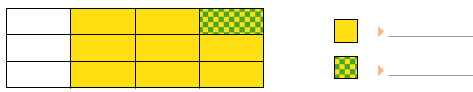
\includegraphics[scale=.6]{Images/fraccion.png}
   \end{center}
   \noanswer[.25in]
 \item Encierre todas las fracciones o números mixtos equivalentes a la fracción dada en cada caso
 \begin{enumerate}
 \item $\dfrac{4}{8}$ $\qquad$ $\dfrac{2}{6}$, $\dfrac{2}{16}$, $\dfrac{1}{2}$, $\dfrac{20}{40}$, $\dfrac{5}{24}$, $\dfrac{16}{32}$
 \newpage
 \item $\dfrac{7}{2}$ $\qquad$ $3\frac{2}{6}$, $\dfrac{9}{27}$, $\dfrac{1}{3}$, $\dfrac{21}{6}$, $\dfrac{14}{4}$, $3\frac{1}{2}$\noanswer[.1in]
 \item $\dfrac{2}{3}$ $\qquad$ $\dfrac{4}{6}$, $\dfrac{8}{12}$, $\dfrac{20}{30}$, $\dfrac{14}{15}$, $\dfrac{18}{27}$, $\dfrac{16}{18}$ \noanswer[.1in]
 \end{enumerate}
  \item Amplifica o simplifica las siguientes fracciones. Luego, representa gráficamente el resultado.
\begin{center}
 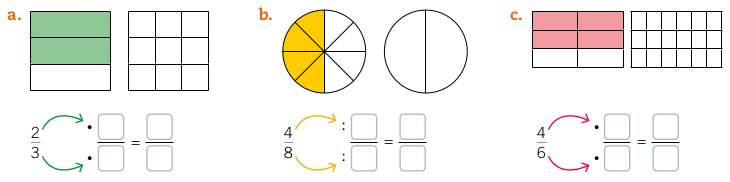
\includegraphics[scale=.4]{Images/AmpSimpFracc.png} 
 \end{center} 
 \noanswer
 \item \begin{minipage}{.6\textwidth}
 Marcela está distribuyendo huevos en cajas de cartón. En cada caja caben 6 huevos y, hasta ahora, Marcela ha llenado una caja y ha puesto 2 huevos en otra.  
 \end{minipage}\hfill
\begin{minipage}{.4\textwidth}
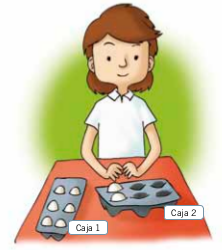
\includegraphics[scale=.4]{Images/Marcela.png} 
\end{minipage}
Complete con los números que faltan en cada caso.
\begin{center}
 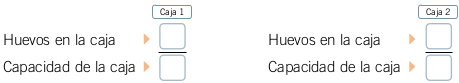
\includegraphics[scale=.5]{Images/Huevos.png} 
\end{center}
 \noanswer

 \end{enumerate}

\end{document}
